\section{Virtual Memory}

\subsection{Page Table Structure}

\begin{figure}[h]
    \centering
    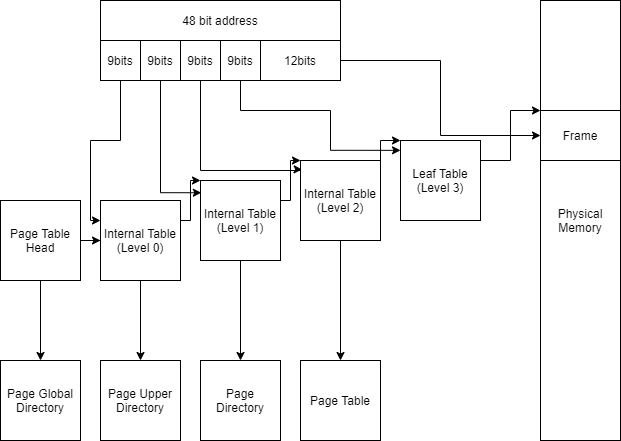
\includegraphics[width=100mm]{page_table.png}
    \caption{Page table structure}
    \label{fig:page_table}
\end{figure}

\noindent
Our page page is structured very similarly to the hardware
page table structures on the ARMv8-A architecture.
There are 4 levels of tables, each containing 512 entries.
Similar to the ARMv8-A architecture, 48 bit virtual addresses
are broken up into series of bits and then used to index
into the page table structures. The last 12 bits are used
as the offset into the physical frame backing the virtual memory.
\\

\noindent
Each entry in the page table is also responsible for keeping track
of the seL4 memory management structures.
As shown in the diagram, the head of the page table maintains
references to the Page Global Directory and each entry in level 0
maintains a reference to a Page Upper Directory etc.
\\

\noindent
Entries in internal and leaf table all have this structure

\noindent
\{ \par
    seL4\_CPtr cap : 39; \par
    frame\_ref\_t frame : 19; \par
    bool valid : 1; \par
    bool init\_pte: 1; \par
    bool readonly: 1; \par
    bool never\_execute: 1; \par
    bool data\_in\_elf: 1; \par
    unsigned char ut\_bit : 1; \par
\noindent
\}

\noindent
Some fields serve slightly different roles in internal and leaf entries
\\

\noindent
In internal entries, the 'frame' field is a reference to the memory backing
the table that this entry points to. In leaf entries, the 'frame' field
is a reference to the memory backing the virtual memory in consideration.
\\

\noindent
In both types of entries, the valid field indicates whether there is memory
currently backing the entry. For internal entries this value will always be true
after memory has been allocated to back the entry as page table frames
don't get evicted in our implementation. For external entries however
valid entries may become invalid when the physical frames they reference
are allocated to other entries.
\\

\noindent
The init\_pte field is used to ensure that read/write/execute permissions
for frames can only be set when they are initially loaded.
\\

\noindent
The readonly and never\_execute fields are only for leaf entries and
specify permissions for a particular frame.
\\ 

\noindent
The data\_in\_elf field impacts how the 'cap' field is interpreted in leaf
entries. If data\_in\_elf is true, this indicates that the contents of the frame
backing this entry should be identical to a corresponding location 
in the elf file.
\\

\noindent
The cap field serves a variety of purposes. In internal entries, it is a
seL4\_CPtr to a seL4-managed memory structure. In external entries, its
interpretation is dependent on whether data\_in\_elf is true. If data\_in\_elf
is false and cap is non-zero, then it is an index in the pagefile to the memory
backing the current entry. If data\_in\_elf is true, then the cap field
is an offset into the elf file for this program from which the data should
be loaded in.
\\

\subsection{Modifications to the Frame Table Structure}

We add the following fields to the frame entry table structure: 

\noindent
\{ \par
    bool no\_evict : 1; \par
    bool used : 1; \par
    bool dirty : 1; \par
    bool unused : 1; \par
    seL4\_ARM\_Page user\_page\_cap : 36; \par
    frame\_ref\_t frame\_and\_entry\_index : 28; \par 
    \noindent
\}

\noindent
The no\_evict field indicates whether a frame can be evicted by the
page replacement algorithm. Frames backing internal page table entries
and ipc buffers are always not evictable. A frame on which IO operations
are being done is also marked as not evictable to avoid race conditions.
It should be noted that since IO is done frame-by-frame, this will not
lead to the situation where all frames could get marked as not evictable
when processing a large buffer.
\\

\noindent
The used and dirty bits are used to implement demand paging.
\\

\noindent
The no\_evict, used, dirty and user\_page\_cap fields could be stored
inside the page table entries, but we reason that it is preferable to 
increase the size of frame table entries which increase in number
linearly with the size of physical memory being managed, rather than
in page table entries which increase with the number of processes and
the amount of memory that the process has touched. Also, in this way, 
we only have two maintain two capabilities to physical frames managed by
the frame table. One for SOS, and another for the user process which
currently has access to the frame.
\\

\noindent
The 'frame\_and\_entry\_index' field is a reference to the page table entry that
currently owns the frame. It is used by the page replacement algorithm
to invalidate page table entries when the frames backing the memory they reference
are paged out and allocated to someone else. 
As depicted above, this field is 28 bits long. The first
19 bits is a reference to a frame in the frame table, and the last 9 bits
index to the entry of that frame. It would be possible to simply store
the memory address to the page table entry, but this scheme saves
some space in frame table entries.
\\

\subsection{Data Transfer between User Processes and SOS}

\noindent
The SOS read and write syscalls accept the virtual address of the user
buffer and the number of bytes to process. The request is then processed
frame by frame. SOS consults the page table to find the SOS virtual
address corresponding to the frame and marks the frame as no evict.
The request for IO is then forwarded on to the SOS file server using the
SOS virtual address for the frame. When the file server 
has completed its operation the frame is again marked as evictable.
This process enforces the virtual memory layout outlined below, so
buffers referencing invalid memory result in the syscall failing and
the IO not being completed. Read and write permissions are also enforced
as the permissions for mapped memory are checked before allowing IO. 
\\


\subsection{Demand Paging}

\begin{figure}[h]
    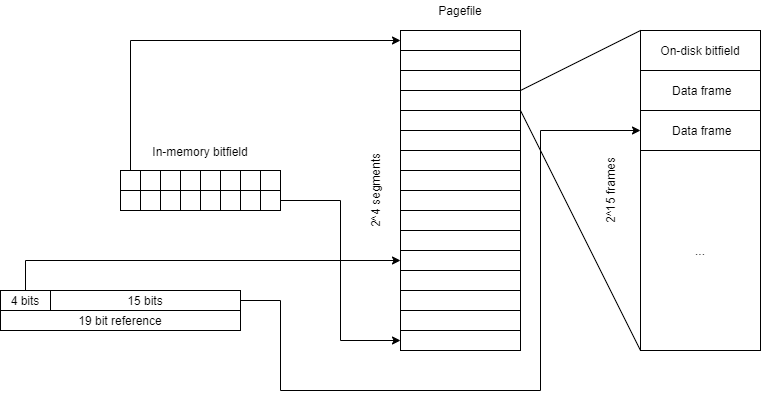
\includegraphics[width=\linewidth]{pagefile.png}
    \caption{Page file layout}
    \label{fig:page_file}
\end{figure}

\noindent
Our pagefile management system is capable managing pagefiles
up to sizes of just over 2GB, as indexes into our pagefiles
19 bit references to 4096-byte pages. The first 4 bits of
these indexes are used to index into a 2 byte bitfield which
is stored in memory. This in-memory bitfield tracks whether 
each of the 16 segments that we break up our pagefile into 
are full or not. The Last 15 bits are used to index into 
the first page of each segment, which itself is a bitfield
used to track whether each page in the segment is in use
or not. So we have a two-level free list, where the first
level is stored in memory and the second level is stored
on disk.
\\

\noindent
We implement the second-chance clock replacement algorithm
as required by the project specification. From our research,
the ARMv8-A architecture does not provide hardware page used
bits so we check whether a page has been used between separate
rounds of the replacement algorithm by un-mapping the page and
marking it and waiting for a VM fault on the page before
un-marking it. We also implement checking pages for dirtiness
in a similar way: all pages are initially mapped in as readonly,
and are marked as dirty if we get a write fault on them.
\\

\noindent
We try to limit writes back to the pagefile as much as possible.
In particular, we never write back pages which are just a copy of
what is in the elf file, and we never write back pages which are
clean and already have an entry in the pagefile.
\\


\subsection{Memory Layout and VM Fault Handling}

\begin{figure}[h]
    \centering
    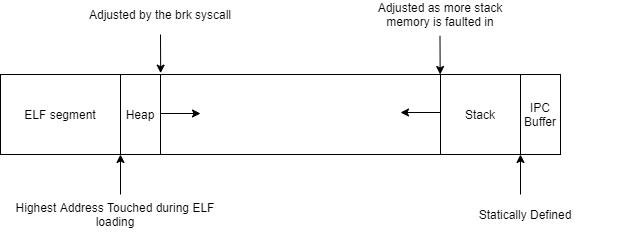
\includegraphics[width=100mm]{memory_layout.png}
    \caption{Process memory layout}
    \label{fig:memory_layout}
\end{figure}

\noindent
Our process memory layout is depicted above. It is quite simple and
makes a couple of assumptions. Our memory layout has four segments.
\\

\noindent
The ELF segment contains all the code and data loaded from the ELF file.
The ELF loader keeps track of the highest address used by the ELF file, 
and after loading is complete, all memory from the bottom of the virtual
address space to this highest address is considered to be the ELF segment.
After loading is complete, any attempts to create new mappings in this
segment will be considered illegal and will result in the process being
killed.
\\

\noindent
The bottom of the heap is the top of the ELF segment. The top of the heap
is dynamically changed by the brk syscall. Attempts to change to top of
the heap so that it intersects with other segments will result in a failed
syscall.
\\

\noindent
The top of the stack is hardcoded to be at a particular address and it
grows down toward the heap as usual. The IPC buffer is fixed in size
and sits above the stack.
\\

\noindent
Attempts to map in memory above the top of the heap and more than a couple
of pages below the bottom of the stack will be considered illegal and
result in the process being killed.
\\

\noindent
An assumption made by our memory layout is that the largest address
touched during ELF loading is sufficiently below the hardcoded top of
the stack so as to allow space for the stack and heap.

